\documentclass[zavrsnirad]{fer}
% Dodaj opciju upload za generiranje konačne verzije koja se učitava na FERWeb
% Add the option upload to generate the final version which is uploaded to FERWeb


\usepackage{blindtext}


%--- PODACI O RADU / THESIS INFORMATION ----------------------------------------

% Naslov na engleskom jeziku / Title in English
\title{Visualization of public transport traffic in real time using the format
	GTFS}

% Naslov na hrvatskom jeziku / Title in Croatian
\naslov{Vizualizacija prometa javnog prijevoza u stvarnom vremenu uporabom formata
	GTFS}

% Broj rada / Thesis number
\brojrada{1246}

% Autor / Author
\author{Luka Miličević}

% Mentor 
\mentor{Prof.\@ Ivana Bosnić}

% Datum rada na engleskom jeziku / Date in English
\date{June, 2024}

% Datum rada na hrvatskom jeziku / Date in Croatian
\datum{lipanj, 2024.}

%-------------------------------------------------------------------------------


\begin{document}


% Naslovnica se automatski generira / Titlepage is automatically generated
\maketitle


%--- ZADATAK / THESIS ASSIGNMENT -----------------------------------------------

% Zadatak se ubacuje iz vanjske datoteke / Thesis assignment is included from external file
% Upiši ime PDF datoteke preuzete s FERWeb-a / Enter the filename of the PDF downloaded from FERWeb
\zadatak{figures/hr_0036543289_73.pdf}


%--- ZAHVALE / ACKNOWLEDGMENT --------------------------------------------------

\begin{zahvale}
  % Ovdje upišite zahvale / Write in the acknowledgment
  Hvala na kavi...
\end{zahvale}


% Odovud započinje numeriranje stranica / Page numbering starts from here
\mainmatter


% Sadržaj se automatski generira / Table of contents is automatically generated
\tableofcontents


%--- UVOD / INTRODUCTION -------------------------------------------------------
\chapter{Uvod}
\label{pog:uvod}

U velikim urbanim gradovima poput Zagreba, javni gradski prijevoz predstavlja neizostavan dio svakodnevnog života. On je temeljni stup mobilnosti, pružajući vitalnu infrastrukturu za povezivanje građana i omogućujući lakše i efikasnije kretanje unutar grada. Velika većina građana svakodnevno koristi javni prijevoz te s obzirom na važnost vremena u užurbanom ritmu gradskog života, dobra organizacija i planiranje putovanja su ključni, jer svi bi htjeli 15 minuta koje potroše na čekanju prijevoza iskoristiti na drukčiji način. Upravo s tim ciljem, ideja završnog rada je stvoriti web aplikaciju, koja pruža stvarno praćenje tramvaja u realnom vremenu, olakšavajući korisnicima efikasno planiranje svojih putovanja, osiguravajući im precizne informacije o dolasku tramvaja i informacijama o pojedinim gradskim linijama prijevoza. Kroz ovaj zadatak, istražit ćemo tehničke izazove s kojima se susrećemo u razvoju takve web aplikacije. Dublje ćemo istražiti ključne elemente koji oblikuju temelje naše aplikacije poput analize API-ja pruženog od strane Zagrebačkog Električnog Tramvaja, proučavanje otvorenih standarda GTFS i GTFS realtime, te detaljniju analizu strukture web-aplikacije, od PostgreSQL baze podataka, backend dijela ostvarenog s node.js i Express.js, do frontend dijela implementiranog s React.js i bibliotekama poput Leaflet.js




%\begin{figure}[htb]
%  \centering
%  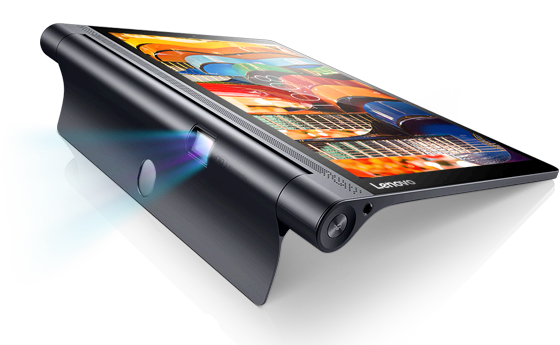
\includegraphics[width=0.38\linewidth]{Figures/lenovo_yoga_tab3_pro_front.png} 
%  \caption{Moja prva slika}
%  \label{slk:prvaslika}
%\end{figure}

%Referenciramo se na sliku \ref{slk:prvaslika} u sredini rečenice, zatim prije zareza %\ref{slk:prvaslika}, te zatim na kraju rečenice \ref{slk:prvaslika}.
%Upravo smo testirali radi li naredba \verb|\ref| ispravno u slučaju kada nakon nje slijedi točka.


%-------------------------------------------------------------------------------
\chapter{Glavni dio}
\label{pog:glavni_dio}

\section{Zagrebački Električni Tramvaj i ulazni podaci}

Zagrebački električni tramvaj, poznatiji kao ZET, je trgovačko društvo koje je u direktnom
vlasništvu Grada Zagreba, te ima ključnu ulogu u organizaciji javnog gradskog prijevoza u Zagrebu.
Posluje od 1910. godine i svakodnevno pruža prijevozne usluge za gotovo milijun ljudi pomoću
tramvaja, autobusa, uspinjače i specijalnih prijevoza. Nedavno je ZET otvorio svoje podatke javnosti
pod Otvorenom dozvolom Republike Hrvatske. Ovi podaci obuhvaćaju GTFS static i GTFS realtime
podatke, koji su trenutno parcijalno implementirani te su dostupni na službenoj stranici ZET-a

etc...

\section[GTFS]{General Transit Feed Specification}

General Transit Feed Specification, kraće GTFS je otvoreni standardizirani format za rasporede
javnog prijevoza i pripadajuće geografske informacije. Široko se koristi diljem svijeta te ga
podržavaju više od 10 tisuća agencija javnog prijevoza u preko 100 zemalja. Neke od platformi koje
koriste GTFS su Google Maps, Apple Maps, Moovit, OpenStreetMap i druge. GTFS je započeo
2005. godine kao ideja za sporedni projekt Googleovog zaposlenika Chris Harrelsona te je danas De
facto standard industrije. GTFS se sastoji od dvije glavne verzije GTFS static (schedule) i GTFS
realtime.

etc...

\subsection{GTFS static}

GTFS static ili GTFS schedule je kolekcija od barem 6 osnovnih, do 26 CSV (comma-separated
values) datoteka s ekstenzijom .txt zapakiranih unutar jedne komprimirane .zip datoteke. Te datoteke
sadrže informacije o rutama, rasporedima, stanicama, i ostalim informacijama o prijevozu. CSV
format pruža otvorenost i jednostavnost rukovanja s datotekama i čini strojno čitanje lakoćom.
Važno je napomenuti da je način kodiranja datoteka imperativan, obavezuje se korištenje UTF-8
kodiranja (podržan je i UTF-8 BOM).

etc...

\subsection{GTFS realtime}

GTFS realtime ili GTFS-rt je ekstenzija GTFS-a koja je nastala 2011. godine te je također de facto
industrijski standard za dijeljenje stvarnih podataka o prijevozu. Jer je GTFS otvoreni standard,
realtime se razvio s ciljem maksimalne interoperabilnosti i lakoće korištenja da bi olakšali
programerima razvoj aplikacija i lakoću dijeljenja informacija o prijevozu između agencija. GTFS-rt
sadrži informacije u stvarnom vremenu o lokacijama vozila, predviđenim vremenima dolaska te
obavijestima o promjenama ruta i otkazivanjima putem web poslužitelja koji koristi protocol buffers
(protobuf). Podaci o stvarnoj lokaciji stvaraju se neprekidno od strane agencije putem sustava za
automatsko praćenje vozila dok se vremena dolaska na odredište izračunavaju korištenjem modela
strojnog učenja koji analiziraju povijesne podatke o položaju i voznom redu

etc...

\section[Protobuf]{Protocol buffers}

Protocol Buffers su jezično i platformski neutralni, proširivi mehanizmi za serijalizaciju
strukturiranih podataka. Razvijeni od strane Googlea, prvotno su bili namijenjeni internoj uporabi,
ali su kasnije postali dostupni pod otvorenom licencijom. Glavni cilj protocol buffera je pružiti
jednostavnost i visoke performanse, te su posebno dizajnirani kako bi bili manji i brži od XML i
JSON formata. Datoteke koje definiraju strukturu podataka u protocol buffer formatu obično imaju
ekstenziju .proto.

etc...

\section{Arhitektura sustava}

Sustav će se temeljiti na modelu Klijent-Poslužitelj. Korisnik će koristiti svoje računalo za pristup
stranici putem web-preglednika, koji će potom komunicirati s mojom aplikacijom koja će se nalaziti
na nekom poslužiteljskom računalu. Frontend dio aplikacije će biti kreiran pomoću React radnog
okvira te će koristiti razne biblioteke koje olakšavaju programiranje različitih funkcija. Taj dio će
korisnik moći vidjeti i koristit će za upravljanje našom aplikacijom. Backend dio će biti kreiran u
JavaScriptu pomoću node.js i raznih paketa poput express.js i drugih. Također u backend dijelu
aplikacije će biti PostgreSQL baza podataka koja će se koristiti za pretraživanje informacija o
rutama koje preuzmemo s ZET-ove stranice.

etc...

\subsection{Baza podataka}

\subsection{Pomoćne skripte}

\subsection{Backend - node.js}

\subsection{Frontend - REACT}

\section{Izgled aplikacije}


%-------------------------------------------------------------------------------
\chapter{Rezultati i rasprava}
\label{pog:rezultati_i_rasprava}


%--- ZAKLJUČAK / CONCLUSION ----------------------------------------------------
\chapter{Zaključak}
\label{pog:zakljucak}


%--- LITERATURA / REFERENCES ---------------------------------------------------

% Literatura se automatski generira iz zadane .bib datoteke / References are automatically generated from the supplied .bib file
% Upiši ime BibTeX datoteke bez .bib nastavka / Enter the name of the BibTeX file without .bib extension

\bibliography{literatura}

%--- SAŽETAK / ABSTRACT --------------------------------------------------------

% Sažetak na hrvatskom
\begin{sazetak}
  Unesite sažetak na hrvatskom.

  \blindtext
\end{sazetak}

\begin{kljucnerijeci}
  prva ključna riječ; druga ključna riječ; treća ključna riječ
\end{kljucnerijeci}


% Abstract in English
\begin{abstract}
  Enter the abstract in English.
  
  \blindtext 
\end{abstract}

\begin{keywords}
  the first keyword; the second keyword; the third keyword
\end{keywords}


%--- PRIVITCI / APPENDIX -------------------------------------------------------

% Sva poglavlja koja slijede će biti označena slovom i riječi privitak / All following chapters will be denoted with an appendix and a letter
\backmatter

\chapter{The Code}


\end{document}
